\label{fs-acker-design}

% \begin{algorithm}
% % $inputs \leftarrow configured\_inputs;$ \\
% % $outputs \leftarrow configured\_outputs;$ \\
% % $acker \leftarrow initialized\_acker;$ \\
% % $random\_generator \leftarrow initialized\_random\_generator;$ \\
% \begin{algorithmic}

% \end{algorithmic}
% \end{algorithm}
% \Procedure{Graph}{$ \alpha, \beta $}    
% \EndProcedure
% % \Upon dsdsd
% % \textbf{Upon} (input) $from \ in\in inputs$

% %     result = process(input.data)

% %     \textbf{foreach} $out\in outputs$ \textbf{do}

% %         out.send(result)

% %         acker.send(\{\})
% \caption{Operator-level algorithm}

\begin{algorithm}
\caption{Operator-side algorithm}
\label{operator_side_algo}
\begin{algorithmic}[1]
\State $inputs \leftarrow configured\_inputs;$ 
\State $outputs \leftarrow configured\_outputs;$
\State $acker \leftarrow initialized\_acker;$
\State $rand \leftarrow initialized\_random\_generator;$
\State \textbf{Upon} (in\_tuple) $from \ in\in inputs$
\Indent
    \State out\_tuple = \{\}
    \State out\_tuple.id = in\_tuple.id
    \State out\_tuple.payload = process(in\_tuple.payload)
    \State out\_tuple.ack\_val = rand.generate()
    \For{$out\in outputs$}{}
        \State out.send(out\_tuple)
        \State acker.send(\{out\_tuple.id, out\_tuple.ack\_val\})
    \EndFor
    \State acker.send(\{in\_tuple.id, in\_tuple.ack\_val\})
\EndIndent
\end{algorithmic}
\end{algorithm}

\begin{algorithm}
\caption{Acker-side algorithm}
\label{acker_side_algo}
\begin{algorithmic}[1]
\State $inputs \leftarrow configured\_inputs;$ 
\State $subscribers \leftarrow configured\_subscribers;$
\State $checksums \leftarrow Map[Int64 \rightarrow Int64]$
\State \textbf{Upon} (tid, ack\_val) $from \ in\in inputs$
\Indent
    \State $checksums[tid] \gets checksums[tid] \bigoplus ack\_val$
    \If{$checksums[tid] = 0$}
        \For{$subscriber\in subscribers$}{}
            \State out.notify\_complete(tid)
        \EndFor
    \EndIf
\EndIndent
\end{algorithmic}
\end{algorithm}

In this section, we focus on the core concepts of our dependency tracking method. Within the design of this mechanism, we aim at providing the following properties:
\begin{itemize}
    \item Fine granularity of tracking: for each input element (or for each small group of input records), it should be possible to determine when the element has been entirely processed independently from other items.
    \item Operator-level or segment-level locality of tracking: the mechanism should provide independent notifications for various segments of a dataflow.
    \item Notifications order preservation: the order of notifications should not contradict the order of input elements arrival with respect to wall time.
    \item Cyclic dataflows support: our tracking technique should be suitable for cyclic dataflow graphs. This feature substantially extends the applicability of a dependency tracking method.
\end{itemize}
Aside from these semantic properties, we want our method to minimize service traffic to achieve less than quadratic complexity from all the parameters introduced in Section~\ref{fs-acker-motivation}.
Our dependency tracking mechanism is inspired by Apache Storm \acker\ technique~\cite{apache:storm:acker} that we mentioned in the previous section, and to deepen into details of our tracking mechanism, we need to remind the details of Storm Acker algorithm and its properties. 

\subsection{Storm \acker~analysis}
\label{sec:acker-analysis}
In this section we aim to analyse the properties of the Storm \acker\ algorithm. The algorithm can be divided into two parts: operator-side and \acker -side. Operator-side algorithm (Algorithm~\ref{operator_side_algo}) describes extra functionality that each operator in a dataflow must implement~\footnote{This logic can be easily hidden from user interfaces}. \acker\ algorithm (Algorithm~\ref{acker_side_algo}) defines \acker\ agent functionality.

To track the processing of an input element and its descendants down the stream, the algorithm builds a chain of ack calls. Each data item in the processing pipeline is labeled by a random number, and this number (\textit{ack value}) is then sent to a special acker agent twice: on element spawn and after its processing by the next operator in a dataflow graph. The second ack call for the element follows spawn ack calls for all output elements of the processing procedure. 

This trick makes a ``link'' in the ack chain and guarantees that input item processing and all its descendants processing are completed if and only if each \textit{ack value} is sent twice. The latter condition can be easily checked by \acker\ using XOR operation for all acks received from the chain, which will turn into 0. The result of the XOR operation can accidentally become zero, but the probability of this event is controlled by the length of the \textit{ack value}, so it can be neglected in practice~\cite{apache:storm:acker}.

\acker\ scheme suites well for Storm architecture, though it has limitations. The chain of acks covers the whole processing pipeline and needs to be split into segments to track particular parts of the execution graph in order to provide dataflow locality property. Due to the asynchronous nature of a distributed processing, there is a race between chains of acks induced by different elements, and there are no guarantees on order of processing complete notifications. Cyclic execution graphs are supported by \acker\ scheme naturally: the chain length can have arbitrary length.

% \subsection{

% Firstly, each input data item is assigned with a unique label and a 64-bit random number. When an operator transforms elements, it preserves the label but assigns a new random number to the transformed record. All operators send tuples $(label, number)$ on each input and output element to a special agent called \acker . \acker\ XORs all random numbers grouped by the labels. 

% Note that each random number is sent to \acker\ precisely two times: when an operator sends a new transformed element downstream and when the next operator receives it. Therefore, if the XOR checksum for some label becomes zero, it means that all elements with that label are successfully processed. \acker\ broadcasts notifications on these events.

% To avoid checksum becoming zero until all elements with a specified label are entirely processed, operators firstly send tuples $(label, number)$ for output elements and only after that for the input. There is a small probability that the random numbers will be XORed into zero accidentally, but it can be neglected in practice~\cite{apache:storm:acker}.

% We can illustrate \acker\ as a table with two columns: label and checksum. Table~\ref{ack_table} illustrates such table. According to this example, elements with label $b$ have been entirely processed, while records with labels $a$ and $c$ are still in processing.

% \acker\ mechanism provides for the fine granularity of tracking and cyclic dataflows support out-of-the-box. However, only the uniqueness property of labels does not allow \acker\ to support block-level locality and notifications order preservation. Further, in this section, we design a more sophisticated structure of labels. Using these extended labels, we propose a \tracker\ mechanism that complements \acker\ and provides for all desired dependency tracking properties. 

% \subsection{\tracker\ mechanism}

% \begin{algorithm}
%  \KwData{Execution graph $G$, input stream $I$, random number generator $r$, input element $d$}
%  \KwResult{Processing complete notifications}
 
% $tid = r.next()$ \;
% $S = \{(node: G.Source, data: d, tuple: tid, ack: r.next()\}$ \; \\
% \While{$S \ne \emptyset$}{
%  $t = S.Any()$\;
%  $S = S \setminus \{t\}$\;
%  \eIf{$t.node = G.Source()$}{
%   $O = \{t.data\}$ \;
%  }{
%   $O = t.node.process(t.data) $\;
%  }
%  \For{$\forall o \in O, \forall n \in G.Output(t.node)\setminus G.Sink$}{
%     $ack = r.next()$\;
%     $S = S \cup \{(node: n, data: o, tuple: t.tuple, ack: ack)\}$ \;
%     $Ack(t.tuple, ack)$ \;
%  }
%  $Ack(t.tuple, t.ack)$\;
% }

% \eIf{$Ack(tid) = 0$}{
%  $Complete(d)$\;
% }{
%  $Replay(d)$\;
% }
% \caption{Storm acker algorithm}
% \end{algorithm}

\begin{table}
    \caption{Acker table}
    \label{acker_table}
    \centering
    \begin{tabular}{|c|>{\bfseries}c|c|c|} 
      \hline
      Released & TID & XOR & Input timestamp  \\ \hline \hline
      \checkmark & q & 000 & 1 \\ \hline
      & z & 101 & 4 \\ \hline
      \checkmark & d & 000 & 3 \\ \hline
      & p & 110 & 2 \\ \hline
    \end{tabular}
\end{table}

% \acker\ mechanism provides for the fine granularity of tracking and cyclic dataflows support out-of-the-box. However, only the uniqueness property of labels does not allow \acker\ to support block-level locality and notifications order preservation. Further, in this section, we design a more sophisticated structure of labels. Using these extended labels, we propose a \tracker\ mechanism that complements \acker\ and provides for all desired dependency tracking properties. 

\subsection{Notification order preservation}

\begin{table}
\caption{Acker + ordering}
  \label{acker-ordering}
  \centering
  \begin{tabular}{|c|>{\bfseries}c|c|c|c|} 
    \hline
    Released & GT & XOR & Input timestamp  \\ \hline \hline
    \checkmark & 1 & 000 & 1 \\ \hline
    & 2 & 110 & 2 \\ \hline
    blocked by 2 & 3 & 000 & 3 \\ \hline
    & 4 & 101 & 4 \\ \hline
  \end{tabular}
\end{table}
In \acker\ algorithm each input element is identified by so-called \textit{tuple identifier} (\textbf{TID}). In the original algorithm, it is assigned at random when an element enters a system and has no associated semantics. 

Table~\ref{acker_table} illustrates original \acker\ table. As we can note, labels are random and do not correspond to input timestamps. Hence, e.g. notification for element with label $d$ is sent before notification for element with label $p$, despite the fact that $p$ entered a system before $d$.

To preserve the notifications order, we change the \textit{tuple identifier} generation procedure. Instead of random tuple identifiers, we capture information about input elements order. We call such tuple identifiers \textit{global times}. In practice, we use the timestamp of the element arrival time for this purpose.

% To demonstrate the differences between \tracker\ and \acker\ schemes we compared them in Figure~\ref{fig:tracker-acker-comparison}. 

With the introduction of the order on the tuple identifiers, the ack table can be sorted. For each label, we delay the processing complete notification up to the moment when all previous accumulators become zero. This will give us an order preservation guarantee.

Table~\ref{acker-ordering} shows modified \acker\ table ordered by \textit{global time}. Global times, which are used instead of random labels, do not contradict the order of input elements arrival. Notification for element with \textit{global time} 3 is not sent although its XOR is zero because an element with less \textit{global time} (2) is not completed.

% In case of exact time this will give us total order on elements processing, in coarse time the order will be enforced for groups of elements. 

We can use \textit{global time} of different precision. In case of precise physical time, this will give us the same properties as \textit{tuple identifier}, as there will be no collisions between \textit{global times} of input elements. However, with the reduction of the time precision \textit{global time}, it will group elements by their arrival times in small batches of a size that is defined by input items rate and the time precision.

The vital practical question is how to synchronize clocks between source nodes to be able to compare \textit{global time} of elements coming from different sources. This problem is resolved in Section~\ref{fs-acker-impl}, here we skip this discussion and assume that all elements are coming from the single source node, so all global times can always be compared.

In the original algorithm, the output elements of operation always have the same \textit{tuple identifier} as an input element. This strict rule will not allow us to make consistent join operations since sometimes, we need to wait for a matching element to continue processing the current one. For example, if we want to join user click logs with access logs of some web service, we need to wait for the access event for further processing of a click. To overcome this difficulty sending acks is controlled by the user in Storm. Instead of this we allow user to spawn events with \textit{global time} equal or \textit{greater} then one of input element.

% The exact structure of this identifier is discussed in implementation section, Each input element has unique identificator that defines the global order between elements. We discuss the exact structure of such identificator in section \ref{fs-acker-impl}, for now let's assume that it is element ingestion timestamp. We call such identificator Global Time.

% Order preservation property requires that completeness notifications for processed elements are ordered according elements Global Times.
% To enforce such order we: 

% \begin{enumerate}
%   \item Use element Global Time as label in acker table
%   \item Sort entries in acker table according to the Global Time
%   \item Send notifications for zeroed entries only when notifications for all previous lines are send
% \end{enumerate}

% This modification is shown in table \ref{acker-ordering}. Notification for Global Time $1$ still can be sent as there are no elements with less Global Time and it is zeroed that means that all elements with such Global Time are completely processed. In contrast to traditional acker, notification for time $3$can't be sent even if there is zero in XOR column because there are unprocessed elements in dataflow with Global Time $2$.
\subsection{Dataflow locality}

\begin{figure}[htbp]
  \centering
  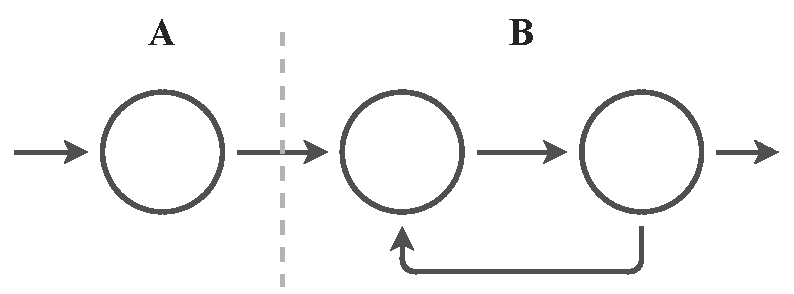
\includegraphics[width=0.3\textwidth]{pics/graph-segments.pdf}
  \caption{Graph segmentation}
  \label{fig:tracker-acker-comparison}
\end{figure}

Notification ordering allows streaming systems to take consistent snapshots and to enforce delivery guarantees. In case when the snapshotting procedure is heavyweight, we want to trigger it as early as possible. For this purpose, we can partition the graph into segments without cycles between them and start snapshotting independently.

To provide segment-wise notifications, we use different \textit{tuple identifiers} for each segment of the graph and introduce the same contract we used to provide order preservation. Downstream segments wait for upstream to send a notification. 

Concluding all our modifications of the \textit{tuple identifier}, it now has two parts: \textit{global time} and \textit{segment identifier}. To send processing complete notification we require:
\begin{enumerate}
    \item XOR accumulator for this identifier to be zero
    \item All segments up the stream do not contain elements with such identifier (local XOR accumulator is zero)
    \item All accumulators for this segment with a  \textit{global time} less than current are nullified
\end{enumerate}

To illustrate the dataflow locality feature, assume that we have a dataflow graph illustrated in Figure~\ref{fig:tracker-acker-comparison}. This graph has two segments: $A$ and $B$. Table~\ref{tracker-table} illustrates \tracker\ table for this case. Notification for \textit{global time} 3 cannot be sent to all subscribers, because elements with \textit{global time} 2 are still being processed. However, local notification for the segment $A$ with \textit{global time} 2 can be sent because all XORS with the prior \textit{global times} for this segment have been nullified and there are no segments up the stream.

Further, in the paper, we reference the complete processing notifications of a certain segment as \textit{min time segment update}. The logic behind this notation is simple after the notification there are no elements with \textit{global time} less or equal to the time of notification left in the stream upper this segment sink.  

\begin{table}
\caption{trAcker}
  \label{tracker-table}
  \centering
  \begin{tabular}{|c|>{\bfseries}c|c|c|c|} 
    \hline
    Released & GT & Segment & Local XOR & XOR  \\ \hline \hline
    \multirow{2}{*}{\checkmark} & \multirow{2}{*}{1} & A & 000 & \multirow{2}{*}{000} \\ \cline{3-4}
    & & B & 000 & \\ \hline
    \multirow{2}{*}{} & \multirow{2}{*}{2} & A & 000 & \multirow{2}{*}{110} \\ \cline{3-4}
    & & B & 110 & \\ \hline
    \multirow{2}{*}{blocked by 2} & \multirow{2}{*}{3} & A & 000 & \multirow{2}{*}{000} \\ \cline{3-4}
    & & B & 000 & \\ \hline
    \multirow{2}{*}{} & \multirow{2}{*}{4} & A & 100 & \multirow{2}{*}{101} \\ \cline{3-4}
    & & B & 001 & \\ \hline
  \end{tabular}
\end{table}

\subsection{\tracker\ overview}

In this section, we introduced the \tracker\ dependency tracking mechanism that is based on the \acker\ technique, but has the following properties:

\begin{itemize}
    \item \tracker\ guarantees notifications order preservation that allows systems that use \tracker\ implement consistent state snapshotting protocol~\footnote{For some systems, it may also need to implement operator input blocking between two sequential notifications, but this change is trivial}.
    \item \tracker\ provides for segment-level locality (or operator-level if dataflow does not contain cycles) that allows systems to implement efficient asynchronous snapshotting protocol~\cite{Carbone:2017:SMA:3137765.3137777}.
    \item Under high input rates and with multiple distributed data sources, labels (\textit{global times}) can be the same for several input elements. In edge cases, it may affect tracking granularity. The probability of XOR collision in these cases can be controlled by the length of the \textit{ack value}.
    \item The amount of service network needed for \tracker\ is the same as for \acker\ - $O(N+C)$, where $N$ is the length of a dataflow, and $C$ is the number of computational nodes. The support of cyclic dataflow remains as well.
\end{itemize}

% depends on all earlier in terms   Acks from segments are appended with segment identifier and acker splits entry for each Global Time into several ones, one for each segment. Though, Ack table \ref{acker-ordering} from previous example transforms into \ref{tracker-table}. Note that Local XORs sums into the global one.

% Completeness notification are sent in the same way as in previous subsection using the same global XOR. Additional segmented notifications are used for consistent snapshotting. They are sent if all entities with the lower Global Time and the same segment are zeroed.

% \ref{graph-segments}


% \subsection{Examples} \label{tracker_examples}
% In this section we show the application of the introduced mechanism to two popular tasks emerging in stream processing: completeness monitoring and state snapshotting. These tasks are usually addressed by different algorithms by \tracker\ allows to solve them both with introduction of a single agent.
% \subsubsection{Completeness monitoring}

% \subsubsection{State snapshotting}
